%% Copyright goes here later.
%%
%% \VignetteIndexEntry{Waterfall Charts in R}

\documentclass[12pt,letterpaper]{article}

\usepackage[style=verbose-trad1]{biblatex}
\usepackage{setspace}

\raggedright
\doublespacing

\setlength{\oddsidemargin}{0in}
\setlength{\textwidth}{6.5in}
\setlength{\topmargin}{-.5in}
\setlength{\textheight}{9.25in}
\setlength{\footskip}{.25in}
\parindent .5in

\title{Waterfall Charts in R}
\author{James P. Howard, II}

\bibliography{waterfall}

\usepackage{/Library/Frameworks/R.framework/Resources/share/texmf/Sweave}
\begin{document}
\maketitle

%% This section initializes the waterfall library and creates three
%% graphs that will appear in throughout the document.

\section{Introduction}

\section{Extended Example}
A picture:\autocite{rasiel:1999}

\setkeys{Gin}{width=0.4\textwidth}
\begin{figure}
\centering  
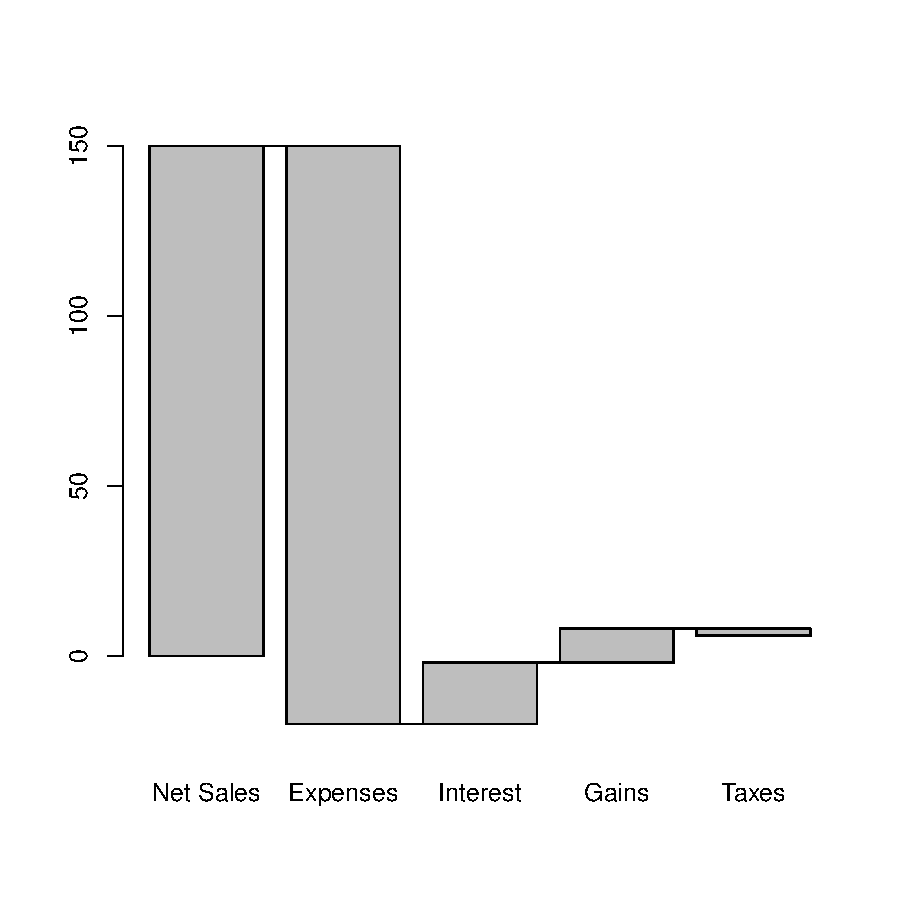
\includegraphics{waterfall-waterfallplot-rasiel}
\caption{Rasiel's Sample}
\label{fig:rasielplot}
\end{figure}

\section{Rationale}

\section{Implementation}

\section{Evaluation}

\section{Conclusion}

\clearpage
\printbibliography

\end{document}
